\chapter{Iqbal Syarif Awalludin (1144095)}
\begin{figure}[!htbp]
  \centering
  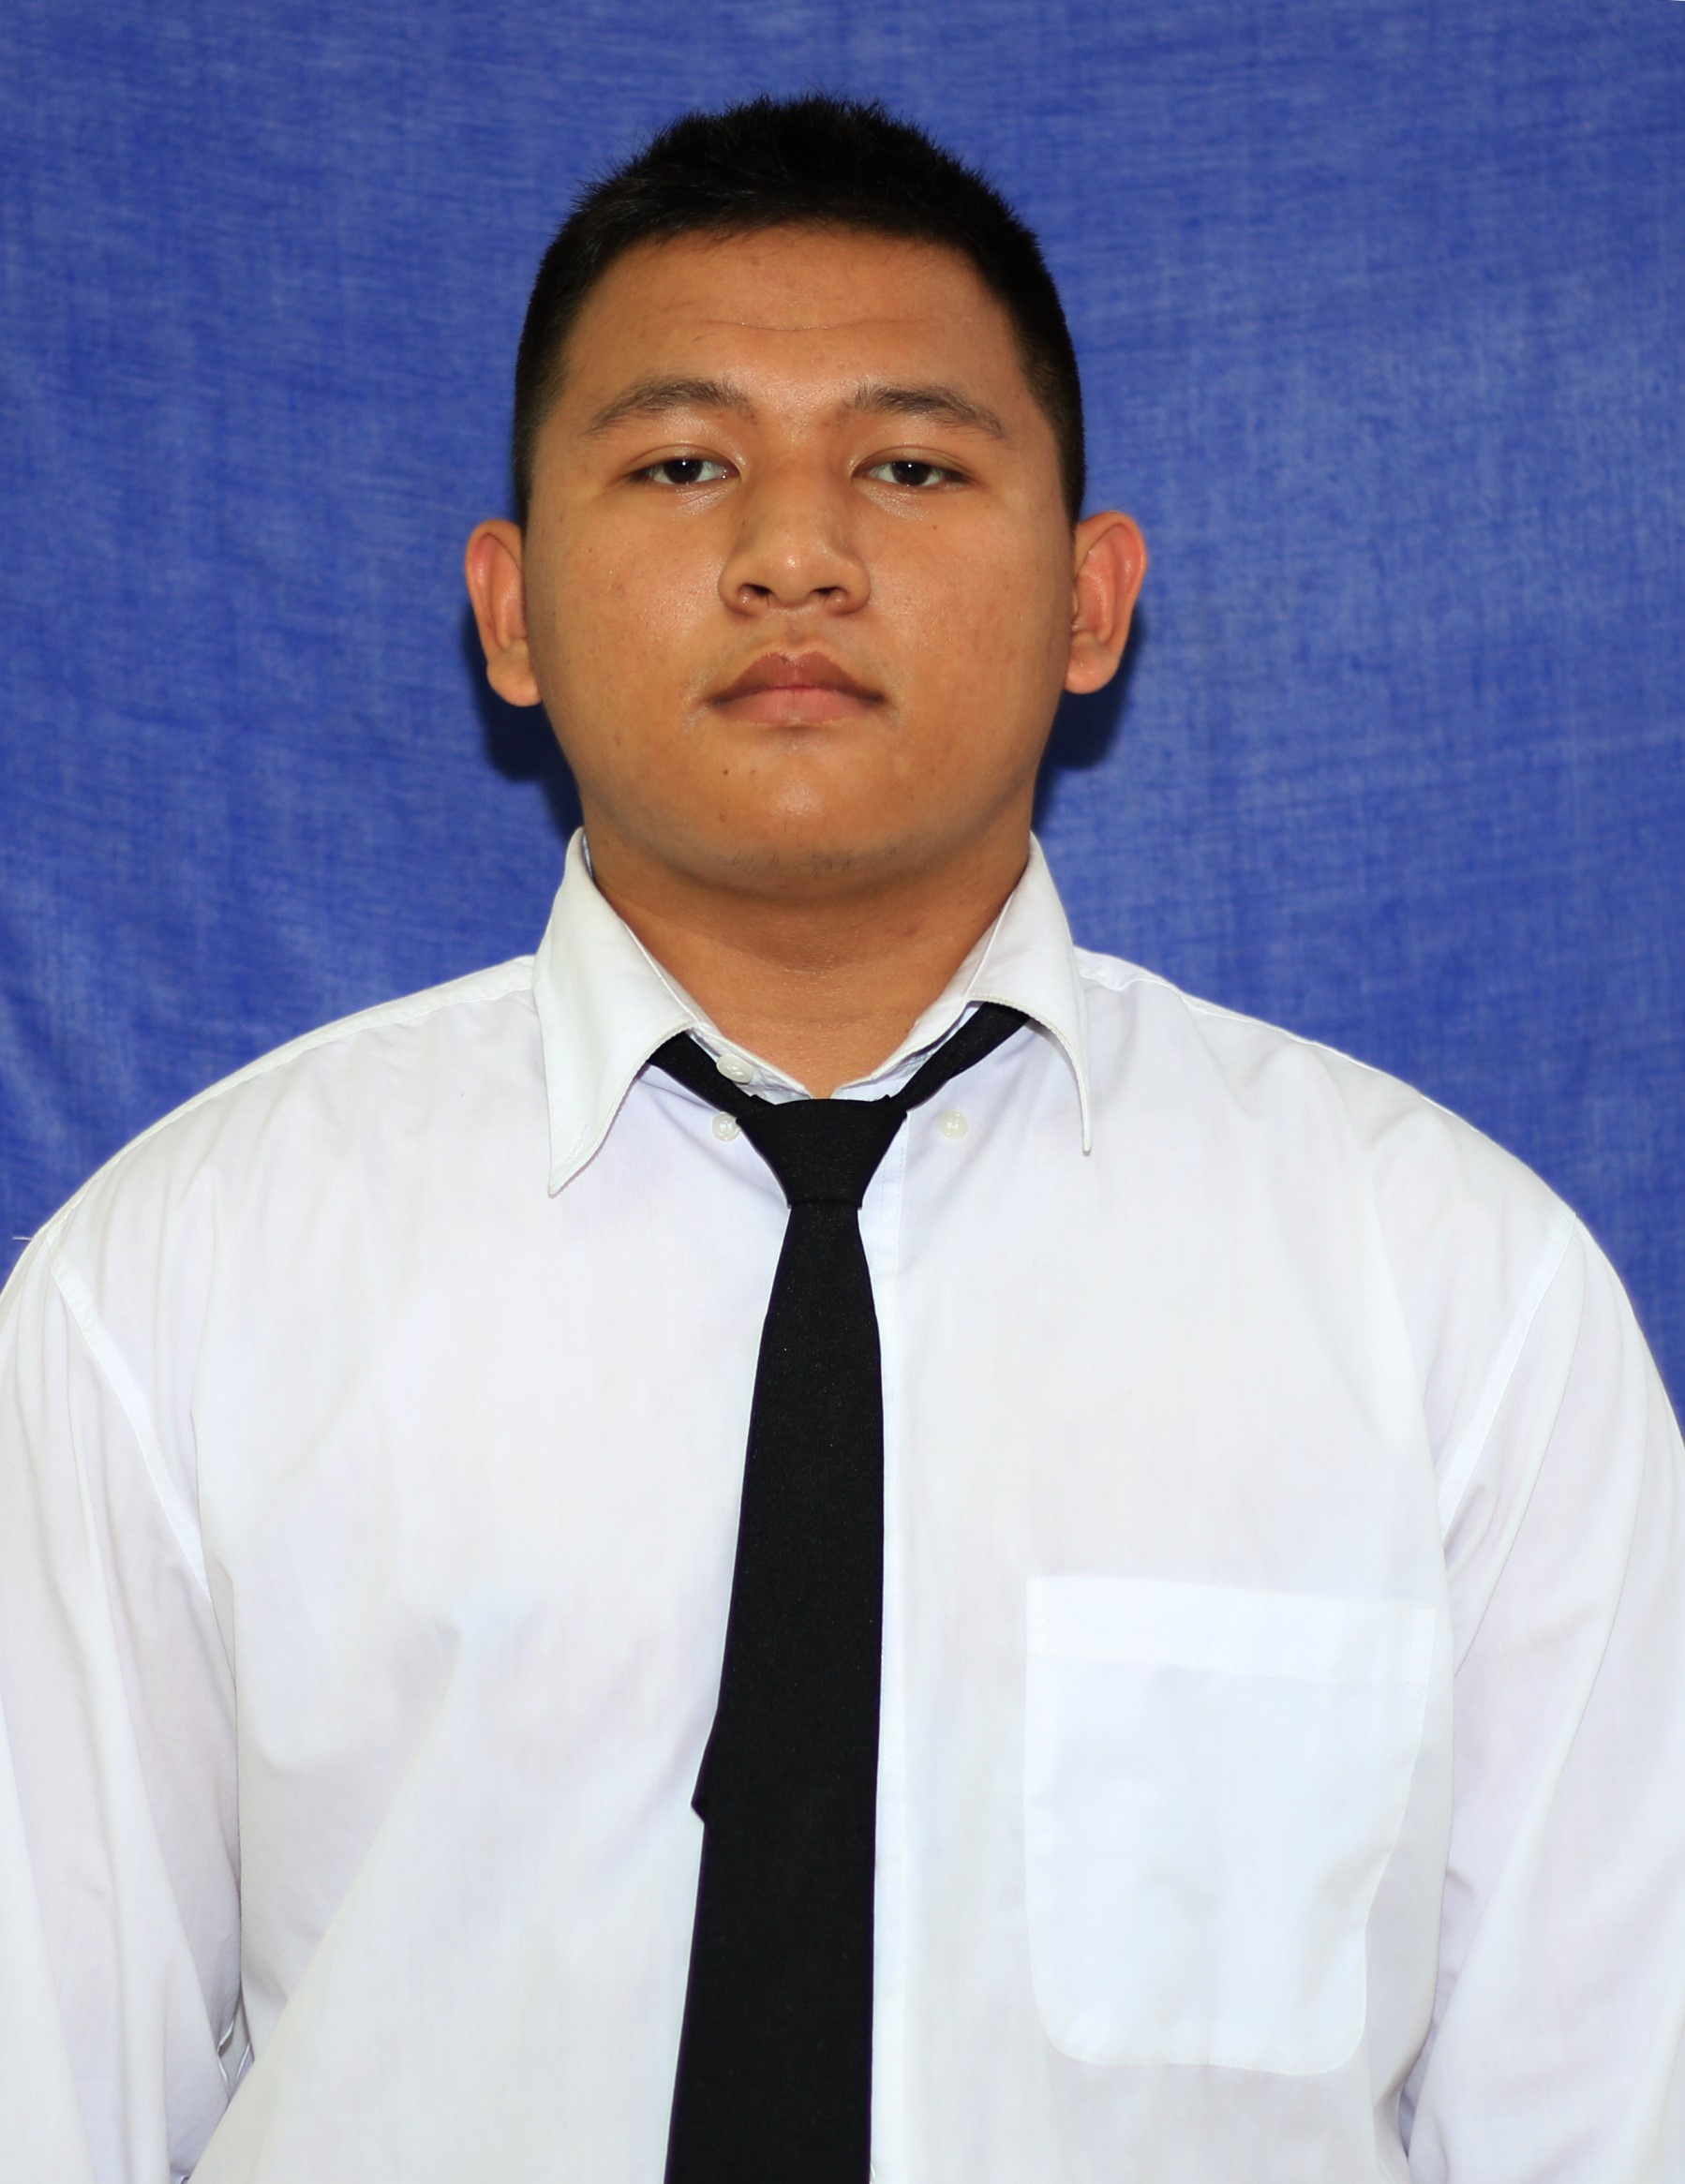
\includegraphics[width=.4\textwidth]{figures/Fotomhs/1144095.jpg}
  \caption{Ini adalah Iqbal Syarif Awaludin}\label{fig:1144095}
\end{figure}
Berikut adalah kegiatan Internship 2 di Prodi D4 Teknik Informatika tertera pada tabel \ref{table:kegiatanharian}
\begin{table}[!htbp]
\centering
\begin{tabular}{ |c|c|c|c|c|c|c|c|c|c| }
\hline
No. & Judul Commit & Baris & Kode Commit & Tanggal \\
\hline
1 & Menambah materi macam2 sensor & (\#42) & 2f5ff92660a69b15c4ea4c4c1fd54a4dcdf02f83 & 25/02/2019 \\
\hline
2 & Membuat poster Sistem antrian dan menambah materi Arduino IDE & (\#43) & b9f90a23a64fba1616df40096016e833c9609e78 & 26/02/2019 \\
\hline
3 & Mengedit buku IOT khususnya bagian Software, Mengedit Laporan2019 khususnya rekomendasi kelulusan dan penilaian & (\#2) & ace406d89cdb4a64623650a1f3b4c8aa4e223635 & 27/02/2019 \\
\hline
\end{tabular}
\caption{Tabel Kegiatan Harian}
\label{table:kegiatanharian}
\end{table}
\subsection{28/02/2019}
\begin{enumerate}
  \item Evaluasi mingguan dari jam 9 pagi s/d istirahat.
  \item Koreksi Laporan Proyek 2 Mahasiswa pada format laporan baik itu margin, EYD, dan Typo pada pukul 15.25 s/d 15.40 .
  \item Menambah materi installasi IDE pada Arkom2019 \#44 pada pukul 15.00 s/d 15.25
  https://github.com/BukuInformatika/Arkom2019/commit/e2c587aa9be2382dc0701bda0a4839f6556289ee
  \item Membantu memperbaiki error merge dan conflict pada saat akan pull request milik Daniel S.P. pada pukul 16.40 s/d 17.00.
  \item Merapikan kembali Meja Ibu Noviana pada pukul 17.00.

\end{enumerate}

\subsection{01/03/2019}
\begin{enumerate}
  \item Absen pada pukul 08.57 pagi.
  \item Mengupdate dan memperbaiki penulisan \textbf{chapter1.tex} pada Laporan2019 pada pukul 09.30.
  \item Membantu memperbaiki error merge dan konflik pada saat akan pull request milik Daniel S.P. pada pukul 10.00 s/d selesai.
  \item Mendiskusikan prihal materi tambahan untuk manajemen konflik di git bersama dengan Pak Rolly pada pukul 11.00.
  \item Sosialisasi Internship 2 pukul  14.00 s/d selesai pukul 16.00
  \item Membantu mengabsen peserta sosialisasi Internship 2 selama sosialisasi berlangsung.
  \item Menambahkan materi manajemen konflik yang sudah disetujui oleh Pak Rolly pada pukul 16.05 sampai selesai.
  \par https://github.com/isawaludin/git/commit/6659fa8d574149a084658e88699e7c24531112d0
  \item Merapikan kembali Meja Ibu Noviana pada pukul 17.00.
  \item Pulang pada pukul 17.05 sore.

\end{enumerate}

\subsection{01/03/2019}
\begin{enumerate}
  \item Absen pada pukul 08.57 pagi.
  \item Mengupdate dan memperbaiki penulisan \textbf{chapter1.tex} pada Laporan2019 pada pukul 09.30.
  \item Membantu memperbaiki error merge dan konflik pada saat akan pull request milik Daniel S.P. pada pukul 10.00 s/d selesai.
  \item Mendiskusikan prihal materi tambahan untuk manajemen konflik di git bersama dengan Pak Rolly pada pukul 11.00.
  \item Sosialisasi Internship 2 pukul  14.00 s/d selesai pukul 16.00
  \item Membantu mengabsen peserta sosialisasi Internship 2 selama sosialisasi berlangsung.
  \item Menambahkan materi manajemen konflik yang sudah disetujui oleh Pak Rolly pada pukul 16.05 sampai selesai.
  \par https://github.com/isawaludin/git/commit/6659fa8d574149a084658e88699e7c24531112d0
  \item Merapikan kembali Meja Ibu Noviana pada pukul 17.00.
  \item Pulang pada pukul 17.05 sore.
\end{enumerate}

\subsection{Score Mingguan}
Total score mingguan adalah 15 keterangan seperti pada Tabel \ref{table:scoremingguan}.
\begin{table}[!ht]
\centering
\begin{tabular}{ |c|c|c|c|c|c|c|c|c|c| }
\hline
Kategori & Keterangan Nilai \\
\hline
Dedikasi & 3 \\
\hline
Produktif & 3 \\
\hline
Integritas & 3 \\
\hline
Disiplin & 3 \\
\hline
Loyalitas & 3 \\
\hline
\end{tabular}
\caption{Tabel Score Mingguan}
\label{table:scoremingguan}
\end{table}

\subsection{04/03/2019}
\begin{enumerate}
  \item Masuk pukul 08.55 pagi
  \item Menambah materi manajemen konflik \#12 pukul 09.00 s/d istirahat
  \par https://github.com/BukuInformatika/git/commit/b377a312a6ba75dcbf9046110a43cc8da25ef63d
  \item Masuk setelah istirahat 13.06
  \item Mendiskusikan Repositori baru untuk Internship 2 dan Ta dengan pihak IRC.
  \item Merapihkan kembali meja Bu Noviana pukul 16.55
  \item Pulang pukul 17.00
\end{enumerate}

\subsection{05/03/2019}
\begin{enumerate}
  \item Masuk pukul 08.45 pagi
  \item Mengoreksi Laporan Proyek 1 dan Internship 1 Mahasiswa dari pukul 10.00 s/d istirahat
  \item Masuk setelah istirahat 13.05
  \item Menambah proses install IDE di buku IoT \#9 pukul 15.00
  \par https://github.com/BukuInformatika/IoT/pull/9/commits/e6dae694976bded14b4a6e23baaef0694b01b3bc
  \item Merapihkan kembali meja Bu Noviana pukul 17.00
  \item Pulang pukul 17.00
\end{enumerate}

\subsection{06/03/2019 s/d 08/03/2019}
\begin{enumerate}
  \item Masuk pukul 08.49 pagi
  \item Menyiapkan konsumsi untuk rapat dosen dari pukul 11.00 s/d selesai
  \item Mendiskusikan prihal hasil rapat bersama Pak Rolly dan Pak Harry beserta mahasiswa magang yang lain
  \item Mengoreksi Laporan Proyek 2 Mahasiswa
  \item Mencari jurnal dengan tema yang sama seperti \textit{CNN MRI} atau \textit{Convolutional Neural Networks MRI} dan di\textit{include} kedalam refences.bib atau 1.bib dan di\textit{push} ke github bersama rekan PRODI pukul 16.00 s/d 17.30
  \par https://github.com/isawaludin/JurnalCNNMRI
  \item Merapihkan kembali meja semua dosen pukul 17.30
  \item Pulang pukul 18.00
  \item pull request menambahkan latar belakang di Line Follower Robotic pada pukul 00.21 s/d 01.30 pagi tgl 8
  \par https://github.com/isawaludin/Arkom2019/commit/cd95658d566ab1c50e61948363936e6addc05ec4
\end{enumerate} 

\subsection{07/03/2019}
Bonus Libur Hari Raya Nyepi

\subsection{08/03/2019}
\begin{enumerate}
  \item Masuk pukul 08.53 pagi
  \item Mengoreksi Laporan Proyek 1 dan Internship 1 Mahasiswa dari pukul 10.00 s/d istirahat
  \item Mengisi form pengajuan pembimbing dan judul
  \item Belajar Gitlab dan simulasi
  \item Merapihkan kembali meja Bu Noviana pukul 17.00
  \item Pulang pukul 18.02
\end{enumerate}

\subsection{Score Mingguan}
Total score mingguan adalah 13 keterangan seperti pada Tabel \ref{table:scoremingguan1}.
\begin{table}[!ht]
\centering
\begin{tabular}{ |c|c|c|c|c|c|c|c|c|c| }
\hline
Kategori & Keterangan Nilai \\
\hline
Dedikasi & 3 \\
\hline
Produktif & 2 \\
\hline
Integritas & 3 \\
\hline
Disiplin & 3 \\
\hline
Loyalitas & 2 \\
\hline
\end{tabular}
\caption{Tabel Score Mingguan}
\label{table:scoremingguan1}
\end{table}

\subsection{11/03/2019}
\begin{enumerate}
  \item Masuk pukul 08.43 pagi
  \item Membongkar dan Membersihkan laptop pribadi
  \item Pull Request ke Laporan2019 tentang report dan score mingguan \#56 s/d istirahat
\par https://github.com/D4TI/Laporan2019/commit/e5e3b17d609662f1cc5cc9e832fa02dc9082d8d7
  \item Menambah materi Miktex dan installasi di Repo Keleketex \#71 dari pukul 12.50 s/d 15.15
\par https://github.com/BukuInformatika/Keleketex/commit/14e98d6915b8dd6d1e8182736c335560f9162912
  \item \textit{Coming Soon}
  \item 
\end{enumerate}
